\section{Case Study: Shopping Carts}
\label{sec:casestudy}

In this section, we use \lang to build two different implementations of a 
shopping cart application.
The first is implemented in a set-oriented style: in the first phase of computation,
changes to the cart are monotonically accumulated and replicated, while in the second
phase (``checkout''), the shopping cart state is summarized and ``sealed'' (finalized).
The second shopping cart design employs an
an imperative, overwriting style: as updates are received, the current shopping cart state
is replaced with a new copy.  We then apply the analysis presented in Section~\ref{sec:properties} 
to analyze both implementations to identify monotonic 
components and state that can be replicated without waiting, and to identify possible
loci of coordination.  Finally, we discuss the potential application of order-restoring
constructs introduced in Section~\ref{sec:stateupdate} to achieve the necessary coordination,
or to provide coordination-free alternatives without synchronization.

\subsection{Implementation based on commutative operations}
An update to the shopping cart is represented as a {\em cart\_action} tuple
containing server and client addresses, a session identifier, an item
identifier, a type field (indicating whether the action represents adding
or removing an item from the cart), and a request identifier to allow
idempotent retry. A checkout request is represented by a {\em checkout}
tuple.  Clients generate {\em cart\_action} and {\em checkout} tuples
and send them to one of the server replicas, determined
by the predicate {\em best\_replica}, whose defining rules are not shown. 
Request identifiers are assigned from a sequence {\em counter}.

\begin{Dedalus}
// client code
sequence[counter, cart_action_stage, 6];

cart_action_stage(Server, Client, Session,
                  Item, Type, ReqId) \(\leftarrow\)
    action(Client, Session, Item, Type, ReqId),
    best_replica(Client, Session, Server),
    counter(ReqId);

cart_action(L, C, S, I, T, R)@async \(\leftarrow\)
    cart_action_stage(L, C, S, I, T, R);

checkout(Server, Client, Session)@async \(\leftarrow\)
    checkout_req(Client, Session),
    best_replica(Client, Session, Server);
\end{Dedalus}

At checkout time, the server computes the difference between the number of
additions and deletions for each item in the cart, and sends a {\em response}
message to the client.

\begin{Dedalus}
// Server code
persist[cart_action, 6];
persist[checkout, 3];

action_cnt(Location, Session, Item,
           Type, count<ReqId>) \(\leftarrow\)
    cart_action(Location, Client, Session,
                Item, Type, ReqId),
    checkout(Location, Client, Session);

status(L, Session, Item, Cnt) \(\leftarrow\)
    action_cnt(L, Session, Item, "Add", Cnt),
    notin action_cnt(L, Session, Item, "Del", _);

status(L, Session, Item, Acnt - Dcnt) \(\leftarrow\)
    action_cnt(L, Session, Item, "Add", Acnt),
    action_cnt(L, Session, Item, "Del", Dcnt);

response(#Client, Session, Item, Amt)@async \(\leftarrow\)
    status(#Location, Session, Item, Amt),
    checkout(#Location, Client, Session);
\end{Dedalus}

\begin{figure}[t]
\centering
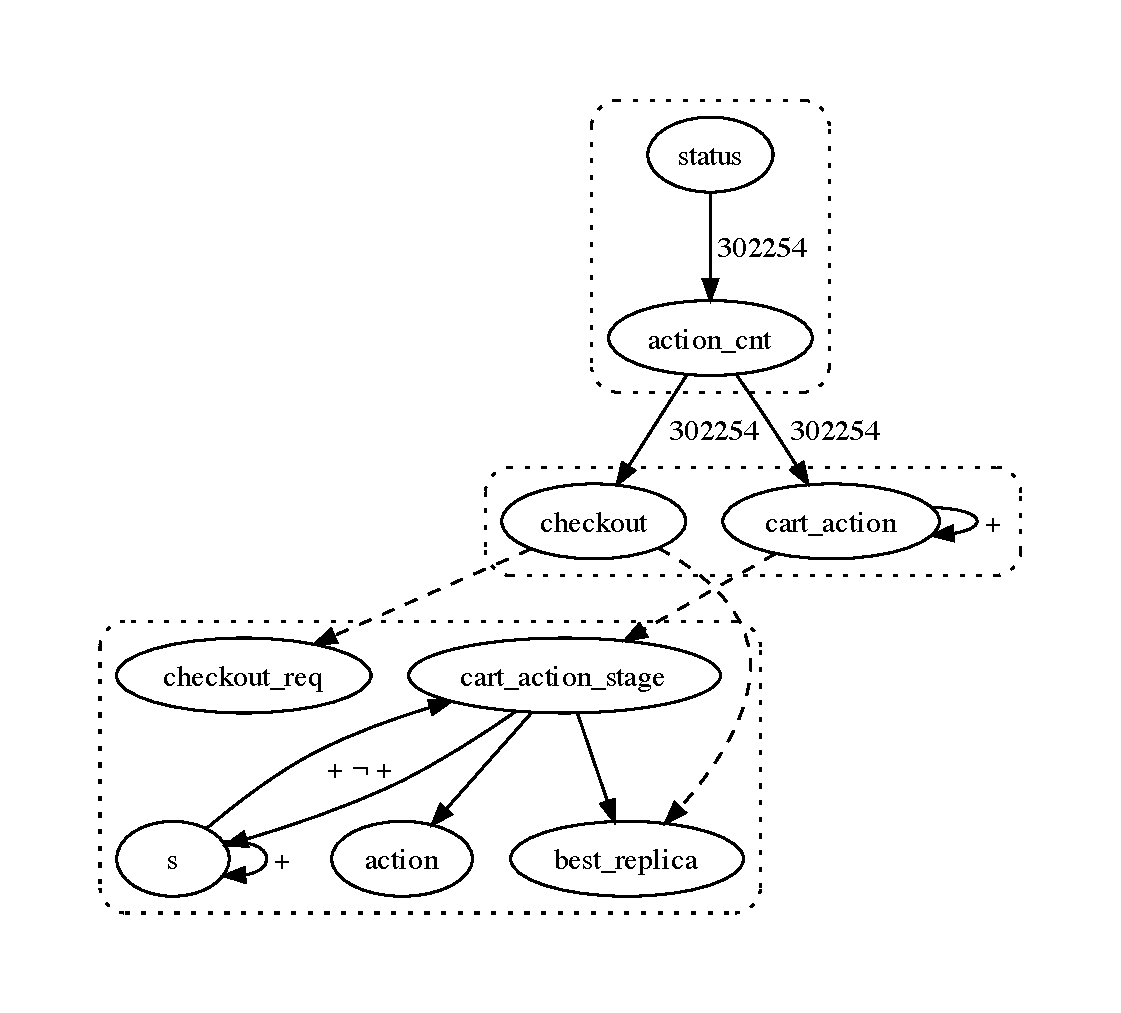
\includegraphics[width=0.9\linewidth]{vizza_brick.pdf}
\caption{PDG diagram for the initial shopping cart program based on commutative updates.}
\label{fig:cs-pgd-1}
\end{figure}

%%Given the PDG diagram for this design (Figure~\ref{fig:cs-pgd-1}),
The PDG diagram generated by our analysis is shown in Figure~\ref{fig:cs-pgd-1}.
The graph nodes are predicates; an arrow indicates a dependency, and a dotted arrow
indicates a dependency via an {\em async} rule.  If the dependency is nonmonotonic
(that is, involving negation or aggregation) it is annotated with a minus (-), and if it is
inductive it is annotated with a plus (+).  Monotonic components are shown boxed with
dotted lines.
Our tests indicate that the program is not necessarily confluent: 
{\em action\_cnt} falls at a point of order, so it may
be affected by the arrival order of tuples to {\em cart\_action} and
{\em checkout}.  This is unsurprising: although both relations are persisted monotonically,
the arrival of a {\em checkout} tuple may cause a universally quantification over {\em cart\_action}
at some time $N$, only to have a subsequent {\em cart\_action} tuple arrive at some time $M > N$.

Depending on the application's requirements, several remedies are possible. If ignoring
late {\em cart\_action} messages is acceptable, then the program must merely ensure
that any latecomers are ignored, and 
%% ---i.e., after a {\em checkout} has occurred, additional
%% {\em cart\_action} messages should 
do not produce additional {\em response} messages.
We can achieve this using the ``at most once'' pattern from Section~\ref{sec:atmostonce}, which ``seals'' the value
of {\em Cnt} in {\em log} at the first insertion. By making the {\em response} message conditional on \emph{log\_event}, we can be sure that only a single response will be sent.

\begin{Dedalus}
commitfirst[log, 4, 3];

log(L, Session, Item, Cnt) \(\leftarrow\) 
    status(L, Session, Item, Cnt);

response(#Client, Session, Item, Amt)@async \(\leftarrow\)
    log_event(#Location, Session, Item, Amt),
    checkout(#Location, Client, Session);
\end{Dedalus}

If ignoring late {\em cart\_action} tuples is unacceptable,
some data dependency between them and {\em checkout} tuples must be established
to ensure that the deduction of {\em action\_cnt} tuples must {\em wait}.  
%%The {\em ordered queue} pattern introduced in Section~\ref{sec:orderinlogic} is one means of %%achieving such an 
%%ordering: if we interpose an ordered queue between {\em cart\_action} and any rules that
%%reference it, we can process the tuples in the order implied by the Reqid field.
%%This strategy would impose an unnecessary ordering on the computation of the aggregate,
%%which we have already shown to be commutative.
%%A more lightweight coordination solution 
One strategy 
is to have the client send a manifest (e.g., a count of total {\em cart\_action} tuples
sent) in the {\em checkout} message:

\begin{Dedalus}
// Client code
stage_cnt(S, C, Se, count<R>) \(\leftarrow\)
  ca_stage(S, C, Se, R);

checkout(S, C, Se, Cnt) \(\leftarrow\)
  stage_cnt(S, C, Se, Cnt),
  checkout(S, C, Se);

// Server code
ca_cnt(S, Se, count<Ri>) \(\leftarrow\) 
  cart_action(S, Se, I, T, Amt, Ri);

response(#C, Se, I, A) \(\leftarrow\)
  status(#S, Se, I, A), 
  checkout(#S, C, Se, Cnt),
  ca_cnt(#S, Se, Cnt);

\end{Dedalus}


In addition to illustrating where a program might require additional coordination, our
analysis also illustrates where coordination is unnecessary.
Note that the predicate {\em cart\_action} is part of a monotonic component that includes {\em cart\_action\_stage}, 
so we can simply and inexpensively replicate it:

\begin{Dedalus}
cart_action(#R, S, I, T, Ri)@async \(\leftarrow\)
    cart_action(#L, S, I, T, Ri),
    replicas(#L, S, R);
\end{Dedalus}

Because {\em cart\_action} is persisted monotonically, it has set semantics over time: at
{\em some} time, when all tuples are received, the order in which they were received is
not important.  Hence asynchronous replication of {\em cart\_action} is confluent,
at least until such time as a nonmonotonic operation is performed on the table.


\subsection{Implementation based on event ordering}

The simplest imaginable shopping cart implementation behaves like a key-value store,
and treats the cart as an opaque object that is repeatedly updated.    Because we have not
attempted to hoist, as we did in the previous example, application logic about cart merging
into the server code, this implementation is superficially more terse and simple.

\begin{Dedalus}
persist[status, 3];
serializer[cart_update, 3, 2];

r1
status(Location, Session, CartObj)@next \(\leftarrow\)
    cart_update(Location,  Session, CartObj);
    
r2
delete status(L, S, C) \(\leftarrow\)
    status(L, S, C), cart_update(L, S, _);
  
response(#Client, Loc, Session, CartObj) \(\leftarrow\)
    status(#Loc, Session, CartObj),
    request(#Loc, Client, Session);

// client code
cart_update(L, S, C)@async \(\leftarrow\) 
    update_event(L, S, C);
\end{Dedalus}

Here, the \dedalus{serializer} macro ensures that updates are
processed one at a time on the server.  Without \dedalus{serializer},
\dedalus{r1} could match multiple tuples in a single fixpoint;
breaking the intended functional dependency between \dedalus{Session}
and \dedalus{CartObj}.

%\paa{no longer sure whether the discussion in the below para is worth the space...}
%Note that 
%{\em cart\_update} is declared using the {\em queue} macro, which expands to
%a program fragment that ensures that tuples corresponding to only one $CartObj$
%are processed in a single fixpoint. \wrm{note that we desire a primary key...}
%Consider the behavior of the program without the queue.  Because {\em
%cart\_update} appears in the head of an asynchronous rule,
%\dedalus{cart\_update} tuples may be assigned arbitrary timestamps, and some
%\dedalus{cart\_update} facts may be assigned the same timestamp, even though
%they were derived serially at the sender.  \wrm{this causes some issue because
%we have a logic bug in our program...}

Figure~\ref{fig:cs-pdg-2} contains a PDG diagram of our
implementation, and reveals a bug.  \dedalus{cart\_update} is in a
different monotonic component than \dedalus{update\_event}; as updates
are propagated from one monotonic component to another, they may be
reordered.  Therefore, the replicas may apply updates in different
orders, and end up with different end-states.

The solution to the problem is simple; we replace the \dedalus{serializer} macro with an \dedalus{ordered queue}.  We entangle the clients' clocks to provide an ordering over the updates:


\begin{figure}[t]
\centering
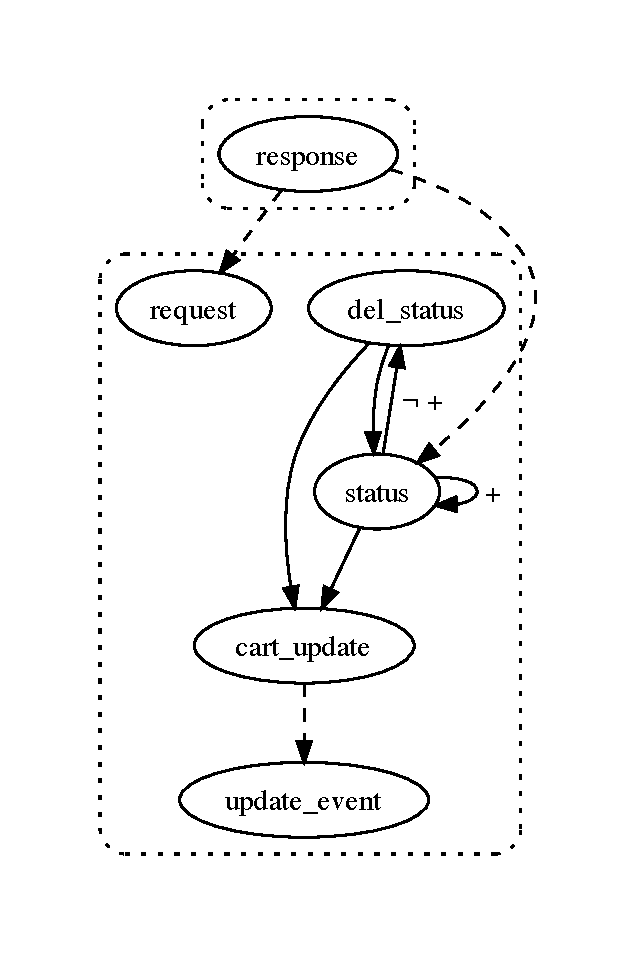
\includegraphics[width=0.65\linewidth]{vizza_straw.pdf}
\caption{PDG diagram for the shopping cart implementation based on ordered events (excluding {\em checkout}).}
\label{fig:cs-pdg-2}
\end{figure}

%Looking at the above program, we can see that {\em status} is defined by the
%state update pattern (Section~\ref{sec:mutable}) on {\em cart\_update}---recall that
%the state update pattern means that the ``latest'' tuple ``wins.'' Thus clearly
%{\em cart\_update} tuples do not commute with each other
%%%, the program is not confluent, 
%and the program as
%given is unlikely to return the correct version of the cart in a {\em response}
%message.  Our PDG analysis confirms this: a stratum boundary separates the client state
%(at {\em update}) from the server state ({\em cart\_update}), upon which all other 
%predicates in the program, including {\em response}, depend.
%
%Considering the {\em cart\_update} tuples in the client's order would solve
%this problem.  However, the client's order of the updates is lost through the
%asynchronous derivations of {\em cart\_update}, which may arbitrarily reorder
%updates.  In Section whatever, we identified the concept of entanglement as a
%way to preserve an order in the face of asynchrony.  We can communicate the
%desired order from client to server by entangling the sender's time in rule
%\dedalus{r4}, and having the server process updates in this order.\footnote{
%We could also have used a sequence, if we wanted more control over the range of ordered
%values.}
%The rest of the code is unchanged, except that an additional argument must be
%added to {\em cart\_update}:

\begin{Dedalus}
cart_update_queue(L, S, C, N)@async \(\leftarrow\)
    update_event(L, S, C)@N;
\end{Dedalus}

%\wrm{the high level point here is that we've made some bad design choices that
%result in us having to over-specify the order.  clearly, a shopping cart doesn't
%need this much order because it's commutative, and indeed, we can write it in a
%much simpler way.  rusty will insert some points here about how distributing
%this naive example results in tons of ugliness (e.g. paxos), and explain that
%yes, we could do that in the language if we want (cite netdb).  this will be a
%nice contrast with later examples which can be distributed much more easily
%because they have much less order and larger monotonic sections.  home run!}

This approach overcomes the nondeterministic ordering implied by asynchronous
communication with brute force: a totally-ordered protocol. This is simple and
inexpensive in this case because it is centralized at the client, obviating the
need for an expensive consensus computation, but the approach has certain
limitations.  First, the client must guarantee that only one {\em
update\_event} is processed per timestep in order to totally order the {\em
cart\_update\_queue} tuples: that is, it must serialize {\em update\_event}
with a queue also.  The matching queues at client and server impose a
synchronization barrier: both sides of the computation must ``spend time''
proportional to the number of tuples.

%\rcs{This might be a good place to cite BFS, sherpa, etc.  The para would go something like this (1) if you want to extend the above to multiple writers, then the ordering construct needs to move to the server side.  (2) Once ordering moves to a master node, you need paxos.  (3) in order to replicate you need to allow replicas to send updates to each other.  If you've settled on per-tuple masters, this probably means some sort of log shipping protocol (a'la our queue, above).  Between the primitives described here and in the bfs/paxos work, you can implement this.  Such systems have been implemented in the past, and are currently in production (CITE PNUTS).  However, such approaches are overkill for shopping carts, and don't show off our nice handling of commutative updates, so:}

\begin{comment}

%\paa{this is too many drawings, but I have to admit I like the drawings and how they illustrate
%the componentization of a distributed system into (hopefully maximally large) 'declarative'
%components that are order-independent and imperative components}

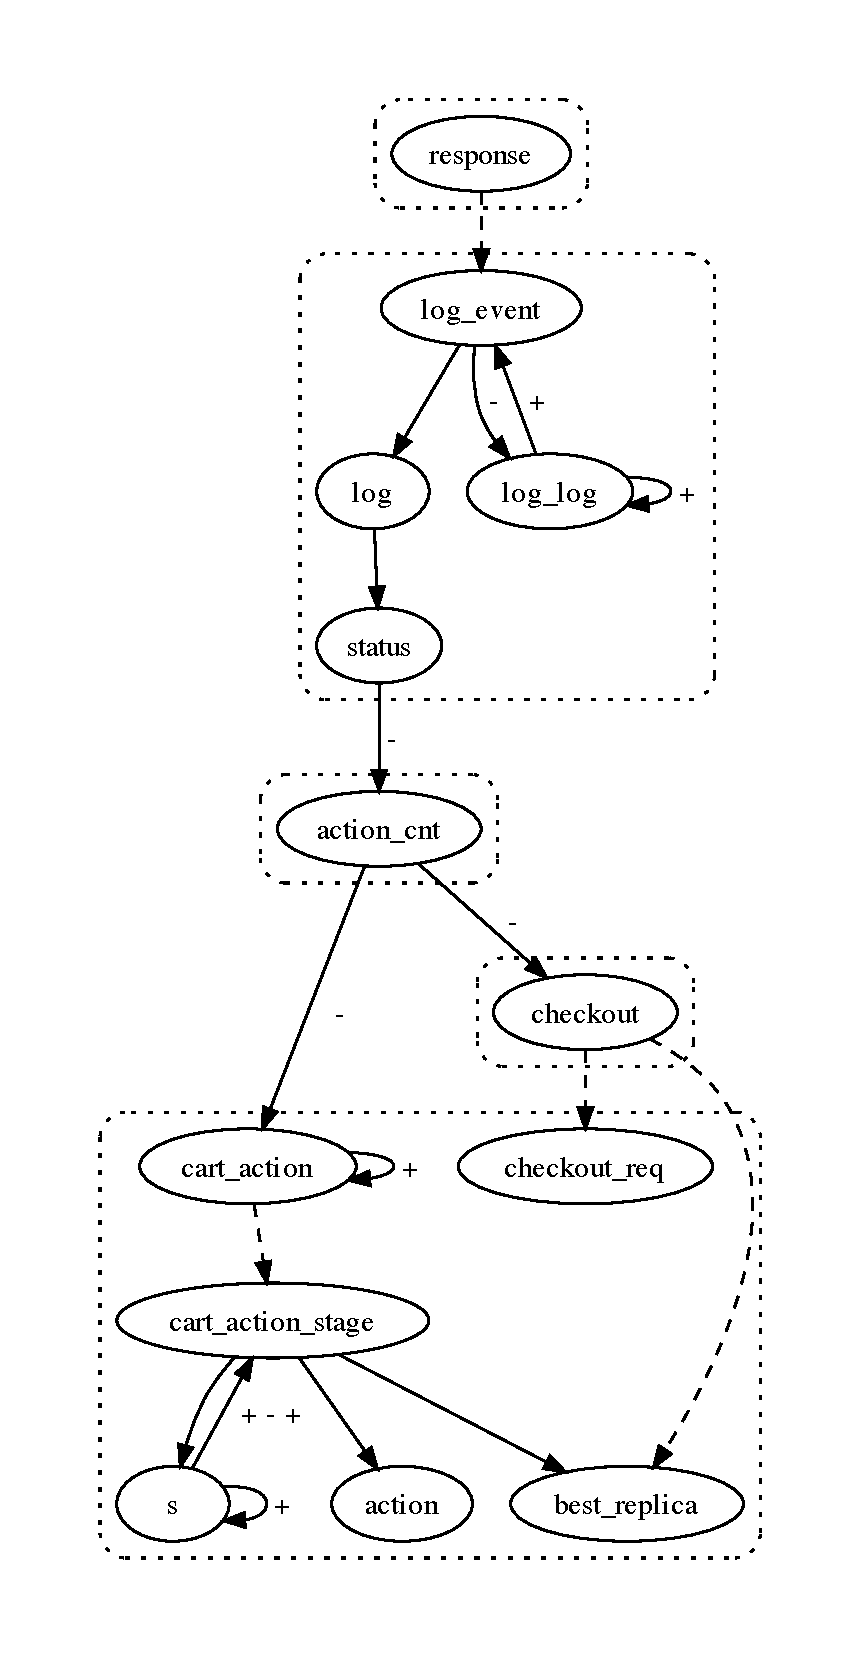
\includegraphics[width=0.65\linewidth]{vizza_withatmostonce.pdf}


\subsection{foo}

... and the client code, just to have it all in here:
\paa{maybe the complete code should just go in an appendix...}

\begin{Dedalus}
commitfirst[publish, 4, 3];

sequence[counter, cart_action_stage, 5];
cart_action_stage(#Server, Client, Session, Item, Type, ReqId) \(\leftarrow\)
    action(#Client, Session, Type, ReqId),
    best_replica(#Client, Session, Server);
    counter(ReqId);

cart_action(#L, S, I, T, R)@async \(\leftarrow\) 
    cart_action_stage(L, #C, S, I, T, R);

checkout(#Server, Client, Session) \(\leftarrow\)
    checkout_req(#Client, Session),
    best_replica(#Client, Session, Server);
\end{Dedalus}
\end{comment}
